%{{{
\documentclass{beamer}
\usetheme{ensam}
\usepackage{pgfplots}
\usepackage{booktabs}
\usepackage{subcaption}
\usepackage{acronym}
\usepackage{tikz}
\usetikzlibrary{calc}
\usepackage{amsmath}
\usepackage {algorithmic}
\usepackage{algorithm}
\usepackage{eqparbox}
\usepackage[font=scriptsize]{caption}
\usetikzlibrary{bayesnet,positioning,calc}
\tikzstyle{obs} = [latent,fill=lightBlue]
\tikzstyle{default}=[draw=sexyRed,thick,rounded corners,text width=0.5in,font=\scriptsize,align=center]
\usepgfplotslibrary{colorbrewer}
\definecolor{ForestGreen}{RGB}{34,139,34}
\newcommand{\comment}[1]{\textcolor{ForestGreen}{#1}}
%algorithmic comment
\renewcommand\algorithmiccomment[1]{%
  \hfill\comment{\#\scriptsize\eqparbox{COMMENT}{#1}}%
}
\renewcommand{\algorithmicrequire}{\textbf{Input:}}
\renewcommand{\algorithmicensure}{\textbf{Output:}}
\title{Independence}
\author{\underline{A.Belcaid}}
\institute{\small ENSA-Safi} 

%tikz bayesian theme
\usetikzlibrary{bayesnet,positioning,calc}
\tikzstyle{obs} = [latent,fill=lightBlue]
\tikzstyle{default}=[draw=sexyRed,thick,rounded corners,text width=0.5in,font=\scriptsize,align=center]
\DeclareMathOperator{\argmin}{argmin}

\pgfplotsset{every tick label/.append style={font=\tiny}}



%acronyms
\acrodef{MRF}{Markov Random Fields}
\acrodef{GNC}{Graduation nonconvexity}


% add bibliography
%}}}

\begin{document}
\maketitle

\begin{frame}
\tableofcontents
\end{frame}

\section{Independence de deux variabbles}

\begin{frame}[t]
  \frametitle{Un simple modele de conditionnement}
  \begin{itemize}
  \small
  \item Lance d'un de \textbf{trucke} avec $\mathbf{P}(H)=p$ et $\mathbf{P}(T)=
    1 - p$.
  \end{itemize}
 \begin{columns}
   \begin{column}{0.4\textwidth}
       \centering
       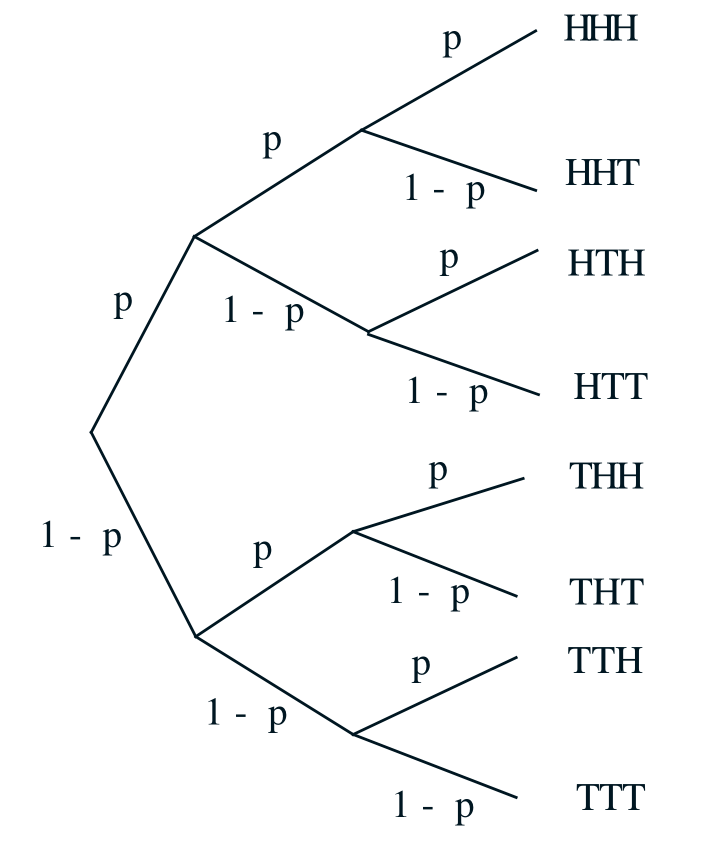
\includegraphics[width=0.8\textwidth]{example_tree_mdel.png}
   \end{column}
   \begin{column}{0.6\textwidth}
    \begin{itemize}
      \scriptsize
      \item Regle de multiplication:
        $$
        \mathbf{P}(THT) = 
        $$
      \item Loi de probabilite totale:
        $$
        \mathbf{P}(\text{Un seul H}) = 
        $$
      \item Regle de Bayes
        $$
        \mathbf{P}(\text{premier lance est H}\;|\;  \text{ 1 seul H}) = 
        $$

    \end{itemize} 
   \end{column}
 \end{columns} 
\end{frame}

\begin{frame}[<+->]
  \frametitle{Independence de deux evenements}

  \begin{columns}
    \begin{column}{0.6\textwidth}
      \begin{itemize}
        \scriptsize
        \item \textbf{Definition intuitive}: $\mathbf{P}(B|A) = P(B)$.
          \begin{itemize}
            \tiny
            \item L'occurence de A nous donne auccune information sur $B$.
          \end{itemize}
        \pause 
          \begin{block}{Definition}
            \scriptsize
            Deux evenements $A$ et $B$ sont \alert{\textbf{independents}} 
            $$
            \mathbf{P}(A\cap B) = \mathbf{P}(A).\mathbf{P}(B)
            $$
          \end{block}
      \begin{itemize}
        \scriptsize
        \item Symmetrique par rapport a $A$ et $B$.\\[8pt]
        \item  Implique directement que  $\mathbf{P}(B|A) = P(B)$.\\[8pt]
        \item S'applique meme si $P(A) = 0$.
      \end{itemize}
            
      \end{itemize}
      
    \end{column}
    \begin{column}{0.4\textwidth}
        \centering
        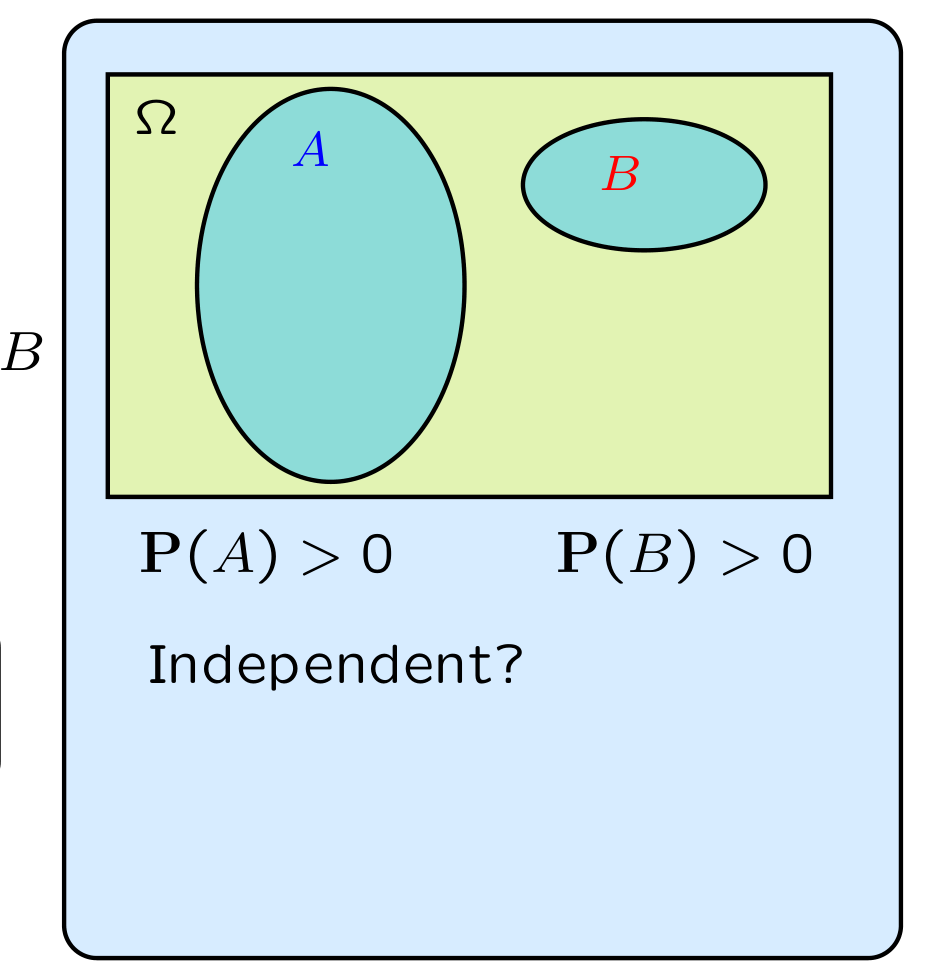
\includegraphics[width=4cm,height=5cm]{test_independence.png}
    \end{column}
  \end{columns}
\end{frame}

\begin{frame}[t]
  \frametitle{Exemples}
 \begin{block}{Exemple 1}
  \scriptsize 
On possede une piece de monnaie truquee qu'on lance deux fois. Dans le premier
lance on peut obtenir soit $H$ soit $T$ avec une probabilite $\frac{1}{2}$.
Cependant le deuxieme lance donne toujours le resultat du lance 1. Ainsi les
deux resultats possibles sont $\{HH, TT\}$.
\begin{itemize}
  \item Est que l'evenement $A=\{\text{H dans le premier lance}\}$ et
    $B=\{\text{H dans le deuxieme lance}\}$ sont independents?
\end{itemize}
 \end{block} 

 \pause
 \begin{block}{Exemple 2}
   \scriptsize
   Soit $A$ un evenement de l'espace d'etats $\Omega$.\\[4pt]
  \begin{itemize}
    \item Est que $A$ et $\Omega$ sont indpendents? \end{itemize}
 \end{block}
\end{frame}

\begin{frame}[t]
  \frametitle{Indpendence deux evenements}
  \small
          \begin{block}{Definition}
            \scriptsize
            Deux evenements $A$ et $B$ sont \alert{\textbf{independents}} 
            $$
            \mathbf{P}(A\cap B) = \mathbf{P}(A).\mathbf{P}(B)
            $$
          \end{block}

          \begin{itemize}
            \item Si $A$ et $B$ sont independents, alors $A$ et $B^c$ sont
              independents?
          \end{itemize}
          \pause
          \begin{eqnarray*}
            P(A) &=& P(A\cap B) + P(A \cap B^c)\\
            P(A)  &=& P(A).P(B)   + P(A \cap B^c)\\
            P(A\cap B^c) &=& P(A) - P(A).P(B)\\
            P(A\cap B^c) &=& P(A).(1 - P(B))\\
            P(A\cap B^c) &=& P(A).P(B^c)
          \end{eqnarray*}

          \pause
          \begin{block}{Mini exercice}
            \scriptsize
            On suppose que $A$ et $B$ sont independents. Est que $A^c$ et $B^c$ sont
            independent?
            
          \end{block}
  
\end{frame}
\section{Independence conditionnelle}

\begin{frame}[t]
  \frametitle{Independence conditionnelle}
 \begin{block}{Definition}
   \scriptsize
   L'independence \textbf{conditionnelle} est definie en utilisant les
   probablites conditionnelles etant donne $P(.\;|\;C)$.
   \begin{equation*}
    P(A\cap B \;|\; C) = P(A\;|\;C).P(B\;|\;C) 
   \end{equation*}
 \end{block} 
 \begin{columns}
   \begin{column}{0.5\textwidth}
      \centering
      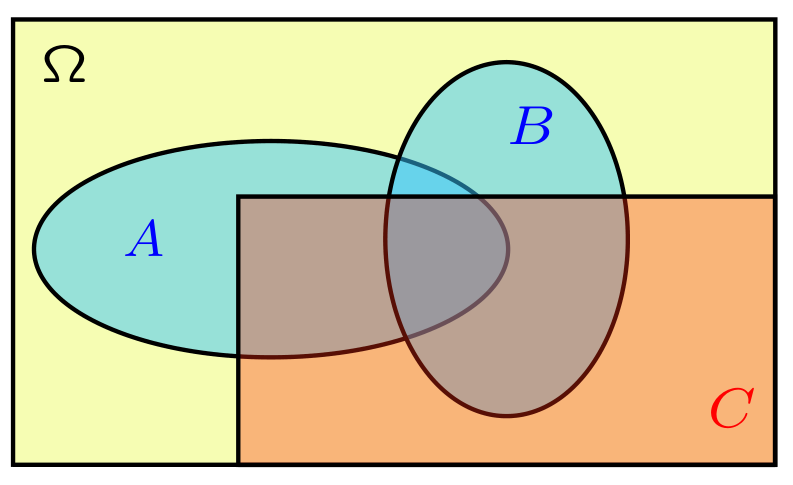
\includegraphics[width=0.8\textwidth]{conditional_independence.png}
   \end{column}
   \begin{column}{0.5\textwidth}
   \begin{itemize}
     \tiny
     \item  On suppose que $A$ et $B$ sont independents.
   \end{itemize}  
   \begin{column}{0.5\textwidth}
      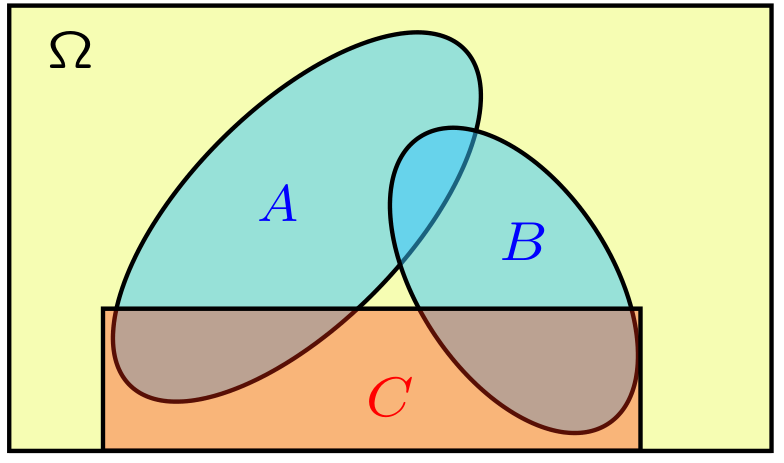
\includegraphics[width=4cm]{independence_vs_conditional.png}
      \begin{itemize}
        \scriptsize
        \item Si $C$ est realise, a t on toujours l'independence?
      \end{itemize}
   \end{column}
   \end{column}
 \end{columns}
\end{frame}
\section{Indepence collection d'evenements}
\begin{frame}[t]
  \frametitle{Independence plusieurs evenements}
 \begin{itemize}
   \small
   \item \textbf{Definition Intuitive}: L'information sur quelque evenements ne
     change par les probabilites des autres evenements.
     \pause
     \begin{block}{Definition}
      \scriptsize 
      Plusieurs Evenements $A_1$, $A_2,\ldots, A_n$ sont dits
      \alert{\textbf{independents}} si:

      \begin{equation*}
        \alert{P(A_i\cap A_j\cap \ldots A_m) = P(A_i)P(A_j)\ldots P(A_m)} .
      \end{equation*}
pour tous les indices distints $i,j,\ldots, m$
     \end{block}
\pause
     \begin{itemize}
       \item \structure{$n=3$?}:
$$
\left\{
  \begin{array}{lll}
    P(A_1\cap A_2) &=& P(A_1).P(A_2) \\
    P(A_1\cap A_3) &=& P(A_1).P(A_3) \\
    P(A_2\cap A_3) &=& P(A_2).P(A_3) \\
    P(A_2\cap A_2\cap A_3) &=& P(A_1).P(A_2).P(A_3) \\
  \end{array}\right.
$$
     \end{itemize}
 \end{itemize} 
\end{frame}
\section{Indepenence deux a deux.}
\begin{frame}[t]
  \frametitle{Indepence et independence deux a deux}

  \begin{columns}
    \begin{column}{0.5\textwidth}
      \begin{itemize}
        \small
        \item Lance deux piece de monnaies:
          \begin{itemize}
            \small
            \item $\alert{H_1}$: premier lance est H.
            \item $\alert{H_2}$: deuxieme lance est H.
          \end{itemize}
          \begin{equation*}
          P(\alert{H_1})=P(\alert{H_2}) =  \frac{1}{2}
          \end{equation*}
          \pause
        \item $\mathbf{C}$: Les deux lances produisent le meme resultat.
      \end{itemize}
    \end{column}
    \begin{column}{0.5\textwidth}
  \only<1->{
    \begin{table}[htpb]
      \centering
      \begin{tabular}{cc}
        \toprule
        HH  & HT\\
        \midrule
        TH & TT\\
        \bottomrule
      \end{tabular}
    \end{table}
  }
    \end{column}
  \end{columns}
  
  \vspace*{1cm}
  \pause
  \begin{itemize}
    \item Est que $H_1$, $H_2$ et $H_3$ sont independents \textbf{deux a
      deux}?\\[8pt]
    \item Est qu'il sont indepenents?
  \end{itemize}
\end{frame}
\section{Quelque problemes}

\begin{frame}[t]
  \frametitle{Probleme des freres du roi.}
 
  \begin{block}{Probleme}
    Un roi vient d'une famille de deux enfants.\\[4pt]
    \begin{itemize}
      \item Quelle est la probabilite qu'il as un seour.
    \end{itemize}
    
  \end{block}
\end{frame}

\end{document}
